In this section I aim to develop an understanding of the differences between various scoring rules and corresponding divergence metrics by visualising the manifold structure they give rise to. For the purposes of illustration here I concentrate only on two-parameter families of distributions such as Gaussian distributions, as these define two-dimensional manifolds which can then be shown in a two dimensional pages of a thesis.

Our goal is to create a two-dimensional map of particular manifolds in such a way that distances measured between points on the map correspond to geodesic distances measured along manifold as precisely as possible. First, it is important to understand that a perfect embedding of this sort does not always exists.

Take the surface of a three-dimensional ball as an example. The sphere is a two-dimensional manifold, which can be parametrised by longitude and latitude. Still, it is impossible to stretch this surface out and represent it faithfully in two dimensional Cartesian coordinate system. This problem -- representing the surface of a three-dimensional object as part of a two-dimensional plane -- is in fact at the core of cartography, and is called \emph{map projection}. When drawing a full map of the surface of the Earth, usually the manifold has to be cut at certain places, but even then, the embedding is only approximate. There are various map projections used in cartography, and the purpose for which the map is used dictates what kind of distortions are tolerable, and what is not.

Understanding that a perfect map of two-dimensional statistical manifolds cannot necessarily be produced, we will resort to approximate embedding techniques developed in the machine learning community. These approximate embedding procedures numerically find a \emph{stretched} manifold in two dimensions that best represents distances on the statistical manifold defined by a particular scoring rule and divergence.

Using numerical isometric embedding techniques developed in the machine learning community, it is possible to visualise the differences between geometries induced by various scoring rules. To do this here we use a techniques called ISOMAP \cite{isomap}.

\begin{enumerate}
\item take a set of probability distributions, preferably so that they relatively densely cover an interesting part of the manifold
\item compute pairwise symmetrised divergence matrix between the selected distributions
\item compute approximate geodesics
\item use metric multidimensional scaling technique embed distributions as points a two-dimensional space
\end{enumerate}

\subsection{Visualising the Shannon-information geometry}

\begin{figure}
	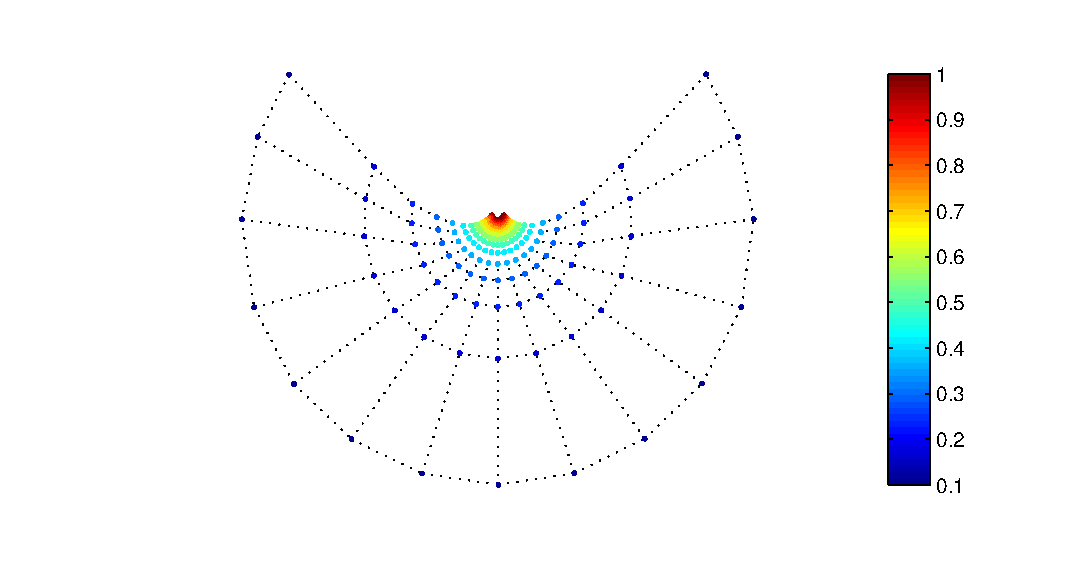
\includegraphics[width=\columnwidth]{figs/embeddings/Normal_KL}
	\caption{Map of Normal distributions on the statistical manifold defined by the log-score, or KL divergence. Dots of the same color show Normal distributions with the same standard deviation. It can be clearly seen that distributions with lower standard deviation are spread out more than those with a higher standard deviation, giving rise to a fan-like structure.}
\end{figure}

\begin{figure}
	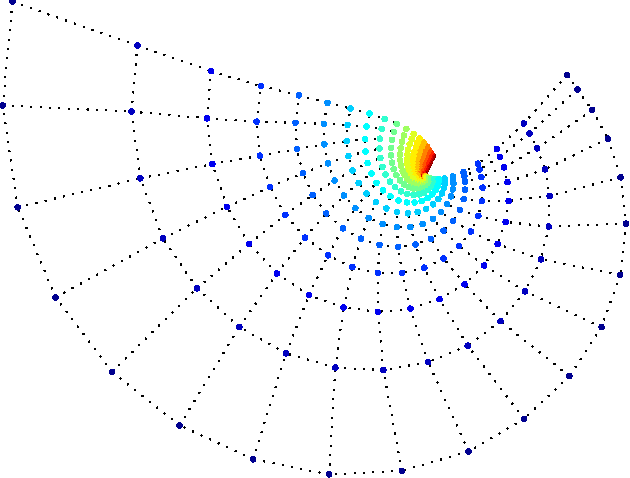
\includegraphics[width=0.45\columnwidth]{figs/embeddings/Gamma_KL_meanvar}
	\hspace{.1\columnwidth}
	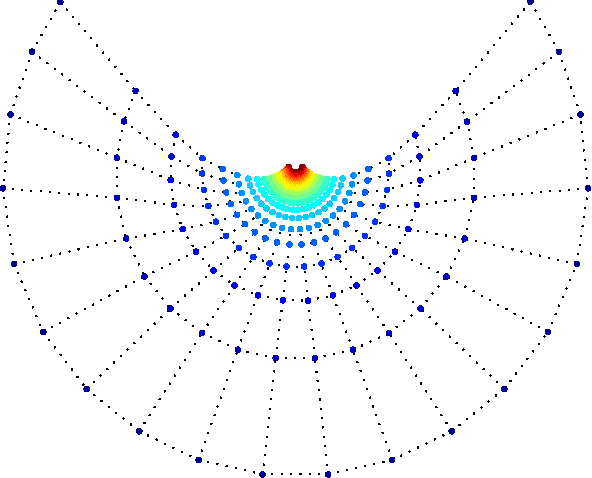
\includegraphics[width=0.45\columnwidth]{figs/embeddings/Normal_KL_nocolorbar}
	\caption{Comparing the statistical manifolds defined by the KL divergence between Gamma \emph{(left)} and Normal \emph{(right)} distributions. Here the mean and variance of each point on the left is matched to the corresponding point on the right (see text for details).  For large values of variance (yellow and red) the two manifolds are very dissimilar, the Gaussian one is symmetric, while the Gamma one is asymmetric. However, as variance decreases (blue), by the central limit theorem Gamma distributions are more alike Gaussians of the same mean and variance, thus the manifold conforms to the fan-like shape that is characteristic of Gaussian distributions.}	
\end{figure}

The most widely used divergence in statistics and machine learning is without doubt the Kullback-Leibler divergence. In his sec I show the geometry it induces on various parametric families of distributions.

Let us start with a very simple, single parameter distribution, the Bernoulli. A Bernoulli distribution describes a binary random variable, where the parameter controls the probability of taking value $1$. In Figure \ref{fig:Bernoulli_manifold} I illustrate the differences between the KL divergence, and the Brier divergence, which corresponds simply to the Euclidean distance between parameter values. As we can see the KL divergence is more sensitive to differences in small (close to 0) and large (close to 1) probabilities, but puts less emphasis on.

When using the KL divergence or the log-score in practical situations, such as in classification, we should therefore expect that much of the statistical power is going to be spent on faithfully matching small probabilities. This is not always desirable: Imagine we were to model the probability that users click on certain news articles on an on-line news website. In this application, most potential clicks have negligible probability, but some user-article combinations may have probabilities closer to $0.5$. If we are to build a recommender system based on this analysis, it is these large probabilities that will be of importance. In this case we are better off using the Brier-score, rather than the log-score which spends serious effort in modelling how small are the small probabilities exactly.

Gaussian distributions are probably the most important family of distributions due to their convenient analytical properties. \TODO{further blah blah about this}
The KL divergence between two univariate Gaussian distributions is available in a closed form and is given by the following formula:

\begin{equation}
	\KL{\Normal_{\mu_1,\sigma_1}}{\Normal_{\mu_2,\sigma_2}} = \frac{\left(\mu_1 - \mu_2\right)^2}{2\sigma_2^2} + \frac{1}{2}\left(\frac{\sigma_1^2}{\sigma_2^2} - 1 - \log\frac{\sigma_1^2}{\sigma_2^2}\right)
\end{equation}


Figure \ref{fig:normals_manifold} illustrates the manifold structure of normal distributions induced by the KL divergence. We can observe that assuming $p$ and $q$ have the same mean, the larger their variance, the easier it becomes to distinguish between them.

We can look at the geometry Shannon's entropy induces within another two-parameter family of continuous distributions, Gamma distributions. Gamma distributions are strictly positive, their probability density function of Gamma distributions is as follows:

\begin{equation}
(x) = \beta^{\alpha}\frac{1}{\Gamma(\alpha)} x^{\alpha-1} \exp(-\beta x)
\end{equation}

where $\alpha,\beta > 0$ are called shape and rate parameters respectively. Special cases of Gamma distributions are exponential distributions when $\alpha=1$.

The KL divergence between Gamma distributions can be computed in closed form and is given by the following formula:

\begin{equation}
	\KL{\Gamma_{\alpha_1,\beta_1}}{\Gamma_{\alpha_2,\beta_2}} = \left(\alpha_1 - \alpha_2\right)\psi\left(\alpha_1\right) - \log\frac{\Gamma(\alpha_1)}{\Gamma(\alpha_2)} + \alpha_1\log\frac{\beta_1}{\beta_2} + \alpha_1\frac{\beta_2 - \beta_1}{\beta_1} \label{eqn:KL_Gamma}
\end{equation}

Figure \ref{fig:Gama_embedding} shows the manifold of Gamma distributions for parameters $a \leq \alpha \leq b, c\leq \beta \leq d$. As we can see this manifold is less symmetric than that of the Gaussians.

For large values of $\alpha$ the standard deviation of the distribution shrinks, and by the central limit theorem, the distribution converges to a Gaussian. We can illustrate this convergence in the manifold structure. For this we first reparametrise the Gamma distribution in terms of its mean and standard deviation. The mean and standard deviation of a Gamma distribution with parameters $\alpha$ and $\beta$ are given by the following formulae:

\begin{align}
	\mu &= \frac{\alpha}{\beta}\\
	\sigma^2 &= \frac{\alpha}{\beta^2}
\end{align}

Solving for $\alpha$ and $\beta$ in these equations we get

\begin{align}
	\alpha &= \frac{\mu^2}{\sigma^2}\\
	\beta &= \frac{\mu}{\sigma^2}
\end{align}

Plugging these into Eqn.\ \eqref{eqn:KL_Gamma} we can now map Gamma distributions with particular mean and variance. Figure 1 compares Normal and Gamma distributions with mean $\mu\in[0.5,1.5]$ and standard deviation $\sigma\in[0.1,1]$. We can observe that as the variance increases, the manifold of Gamma distributions shows a fan-like structure very similarly that of Normal distributions. However, for larger variance, the distributions look less Gaussian, and the manifold becomes more asymmetric. The effect of the central limit theorem would perhaps be even more prominent for smaller values of $\sigma$, but for those cases that case Eqn.\ \eqref{eqn:KL_Gamma} becomes numerically imprecise, as it relies on look-up-table implementation of the Gamma ($\Gamma$) and bigamma ($\psi$) functions.

\subsection{Visualising geometries induced by divergences other than KL}

The main purpose of this section is to visualise differences between the geometries induced by various divergence measures over the same set of distributions. Here we will mainly focus on Gaussian distributions, as it is analytically convenient to compute various divergences between Gaussians in closed form.

A particularly interesting divergence that we will use in subsequent chapters is that based on the kernel scoring rule, called the MMD (section \ref{sec:kernel_scoring}). The kernel scoring rule itself is very flexible, and its properties are dictated by the choice of kernel function.

For several well-known kernels the MMD between two univariate Gaussians can be computed in closed form. For the squared exponential kernel $k(x,y)=\exp(-\frac{(x-y)^2}{\ell^2})$ the divergence is given by the following formula:

\begin{equation}
	\MMD{\Normal_{\mu_1,\sigma_1}}{\Normal_{\mu_2,\sigma_2}} = \ell\left(\frac{1}{\ell+2\sigma_1} + \frac{1}{\ell+2\sigma_2} - \frac{2}{\ell+\sigma_1 + \sigma_2}\exp\left(-\frac{(\mu_1 - \mu_2)^2}{(\ell + \sigma_1 + \sigma_2)^2}\right)\right)
\end{equation}

Figure \ref{fig:Normals_MMD} illustrates the map according to the MMD divergence choosing various values for the lengthscale $\ell$.  \TODO{conclusions} We observe that the structure of the manifold induced by this divergence is qualitatively very similar to that induced by the KL divergence. However, using MMD with the squared exponential kernel allows us the extra flexibility of choosing a characteristic lengthscale, thereby modulating the sensitivity to small differences in variance and mean.

Another widely used kernel is the so-called Laplacian: $k(x,y)=\exp\left(-\frac{\vert x-y\vert}{\ell}\right)$, for which the MMD between Gaussian distributions can still be computed in closed form:

\TODO{find out what the formula is}

Not all scoring rules give rise to smooth manifolds. As an extreme example, consider the following decision problem:

You are uncertain about the temperature of the reactor in a power plant. If the temperature is too high, above a critical temperature $T_{crit}$, the reactor may melt down causing you a loss of \$10 billion. You may choose to shut down the reactor, which costs you \$1 million of lost revenue, irrespective of whether the reactor was indeed overheated or not. You make a probabilistic forecast about the reactor's temperature, and want to make a decision based on that.

This decision rule segments probabilistic forecasts into only two subsets: those which would result in a ``shut down'' decision, and those that result in a ``keep on going''. 

\begin{equation}
	\divergence{reactor}{p}{q} = \left\{
	\begin{array}{cc} 
	    \begin{array}{cc}
	      0        & p(\{t\geq T_{crit}\}) \geq \ell \mbox{ and } q(\{t\geq T_{crit}\}) \geq \ell\\
	      \ell_1 & p(\{t\geq T_{crit}\})  \geq \ell \mbox{ and } q(\{t\geq T_{crit}\}) \leq \ell\\
	      \ell_2 & p(\{t\geq T_{crit}\})  \leq \ell \mbox{ and } q(\{t\geq T_{crit}\}) \geq \ell
	    \end{array}
	\end{array}
	\right.
\end{equation}

This divergence therefore does not give rise to a smooth manifold. Figure \ref{fig two_points} shows a map of Gaussian distributions with respect to the KL divergence. The way $\divergence{reactor}{\cdot}{\cdot}$ segments distributions into ``shut down'' or ``keep on going'' types is also shown. We can make the KL divergence more sensitive to the decision problem at hand by considering a convex combination between $\KL{\cdot}{\cdot}$ and $\divergence{reactor}{\cdot}{\cdot}$.